\documentclass[xetex,14pt,aspectratio=169]{beamer}

\usepackage{caption}
\usepackage[percent]{overpic}
\usepackage{xecyr}
\usepackage{xunicode}
\usepackage[absolute,overlay]{textpos}
\usepackage{fontspec}
\usepackage{calc}
\usepackage{multicol}
\usepackage{hyperref}
\usepackage{setspace}
\defaultfontfeatures{Ligatures=TeX}
\setmainfont{Microsoft Sans Serif}
\usepackage{polyglossia}
\setdefaultlanguage[spelling=modern]{russian}
\newfontfamily{\cyrillicfont}{Microsoft Sans Serif}
\newfontfamily{\cyrillicfontsf}{Microsoft Sans Serif}
\newfontfamily{\cyrillicfonttt}{Microsoft Sans Serif}

\mode<presentation>
{
  \usetheme{Boadilla}      % or try Darmstadt, Madrid, Warsaw, ...
  \usecolortheme{default} % or try albatross, beaver, crane, ...
  \usefonttheme{default}  % or try serif, structurebold, ...
  \setbeamertemplate{navigation symbols}{}
  \setbeamertemplate{caption}[numbered]
  \setbeamertemplate{itemize items}[circle]
  \setbeamerfont{title}{series=\bfseries,parent=structure}
} 

\makeatother
\setbeamertemplate{footline}
{
  \leavevmode%
  \hbox{%
  \begin{beamercolorbox}[wd=.4\paperwidth,ht=2.5ex,dp=1ex,center]{author in head/foot}%
    \usebeamerfont{author in head/foot}\insertshortauthor
  \end{beamercolorbox}%
  \begin{beamercolorbox}[wd=.6\paperwidth,ht=2.5ex,dp=1ex,center]{title in head/foot}%
    \usebeamerfont{title in head/foot}\insertshorttitle\hfill
    \insertframenumber{} / \inserttotalframenumber\hspace*{-8ex}
  \end{beamercolorbox}}%
  \vskip0pt%
}
\makeatletter

\title[Gathering and visualizing flamegraphs in realtime]{On performance analyzing again:\\ {Gathering and visualizing flamegraphs in realtime in Linux environment}}
\author[Alex Chistyakov, DataArt]{Alex Chistyakov, DataArt}
\institute[]{Linux Piter 2016, Russia, SPb.}
\date{}

\begin{document}

\setlength{\fboxsep}{0pt}

\begin{frame}
  \titlepage
\end{frame}

\begin{frame}{Who I am (very quickly)}
\setstretch{1.2}
\begin{textblock*}{\framewidth-0.8cm}(0.0cm,1.5cm) % {block width} (coords)
\begin{itemize}
  \item Senior SW Developer @ DataArt
  \item More than 18 years of professional experience
  \item Researcher @ ISST Lab, ITMO
  \item Used to be a DevOps Engineer and still probably am
  \item Can't quit making presentations w/lots of bullets (that's terrible, I know)
\end{itemize}
\end{textblock*}
\end{frame}

\begin{frame}{Performance optimization is not that hard}
\setstretch{1.2}
\begin{textblock*}{\framewidth-0.8cm}(0.0cm,1.5cm) % {block width} (coords)
\begin{minipage}{\textwidth}
  \centering
  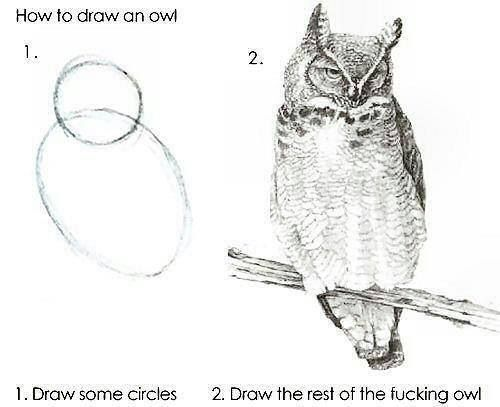
\includegraphics[width=8cm]{img/owl}
\end{minipage}
\end{textblock*}
\end{frame}

\begin{frame}{Ever heard of a 'comfort zone'?}
\setstretch{1.2}
\begin{textblock*}{\framewidth-0.8cm}(0.0cm,1.5cm) % {block width} (coords)
\begin{itemize}
  \item It's crucial to be out of it to learn something new
  \item So I made this presentation in TeX
  \item With lots of bullets, you know
  \item Because I'm not ready yet to leave my comfort zone entirely
  \item Damn, TeX seems to be my new comfort zone ;(
\end{itemize}
\end{textblock*}
\end{frame}

\begin{frame}{Okay, flashback to LP 2015 (w/no bullets)}
\setstretch{1.2}
\begin{textblock*}{\framewidth-0.8cm}(0.0cm,1.5cm) % {block width} (coords)
\begin{minipage}{\textwidth}
  \centering
  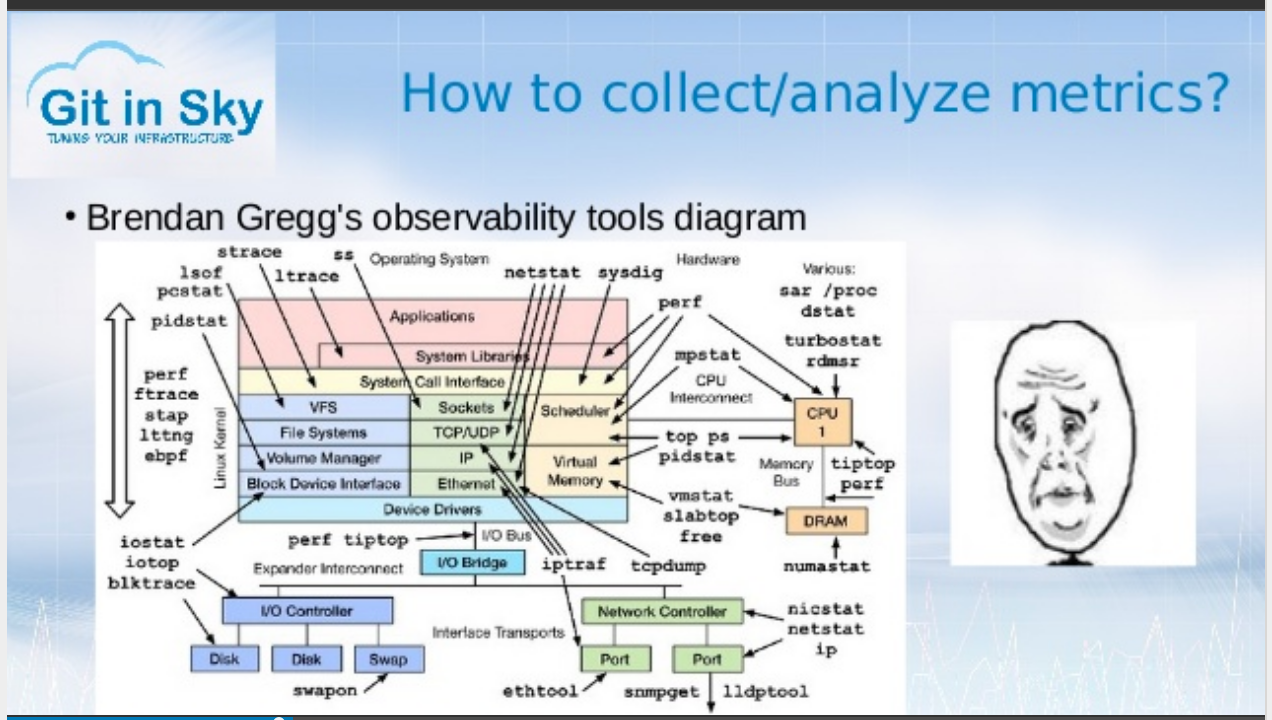
\includegraphics[height=7cm]{img/2015.png}
\end{minipage}
\end{textblock*}
\end{frame}

\begin{frame}{Fast-forward to 2016}
\setstretch{1.2}
\begin{textblock*}{\framewidth-0.8cm}(0.7cm,1.5cm) % {block width} (coords)
Brendan Gregg declared Linux DTrace-complete!
\begin{minipage}{\textwidth}
  \centering
  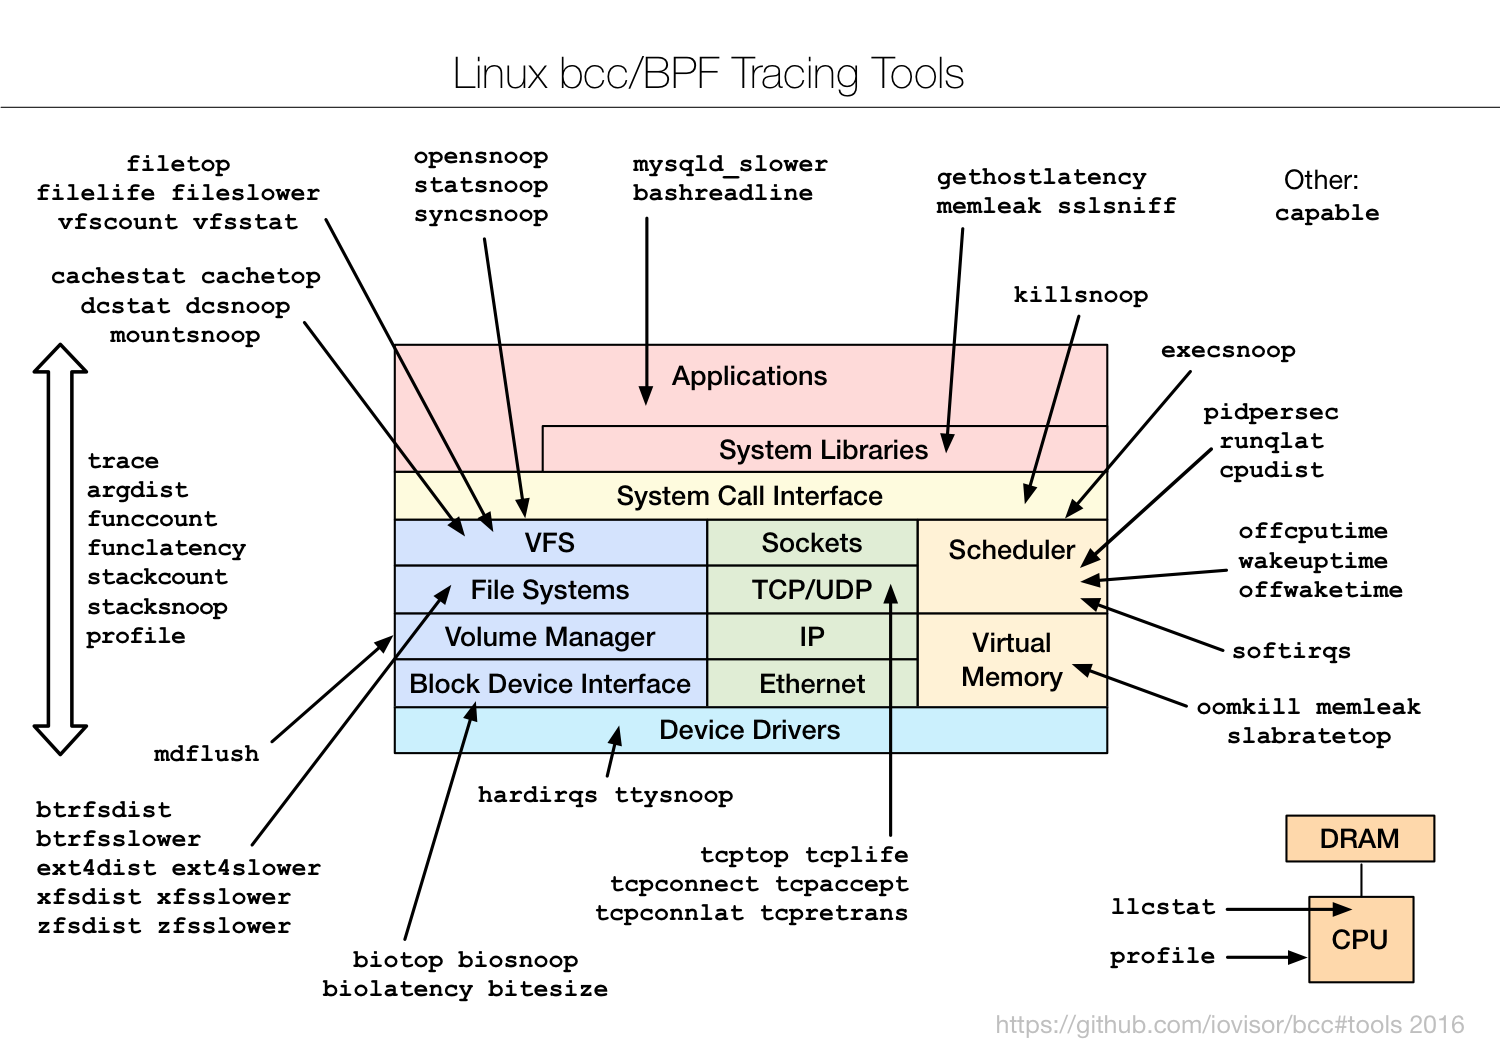
\includegraphics[height=6.6cm]{img/2016.png}
\end{minipage}
\end{textblock*}
\end{frame}

\begin{frame}{A great step forward for mankind...}
\setstretch{1.2}
\begin{textblock*}{\framewidth-0.8cm}(0.7cm,1.5cm) % {block width} (coords)
...but I'm a cat
\begin{minipage}{\textwidth}
  \centering
  
\includegraphics[height=6.6cm]{img/cat}
\end{minipage}
\end{textblock*}
\end{frame}

\end{document}